\documentclass[]{article}
\usepackage{lmodern}
\usepackage{amssymb,amsmath}
\usepackage{ifxetex,ifluatex}
\usepackage{fixltx2e} % provides \textsubscript
\ifnum 0\ifxetex 1\fi\ifluatex 1\fi=0 % if pdftex
  \usepackage[T1]{fontenc}
  \usepackage[utf8]{inputenc}
\else % if luatex or xelatex
  \ifxetex
    \usepackage{mathspec}
  \else
    \usepackage{fontspec}
  \fi
  \defaultfontfeatures{Ligatures=TeX,Scale=MatchLowercase}
\fi
% use upquote if available, for straight quotes in verbatim environments
\IfFileExists{upquote.sty}{\usepackage{upquote}}{}
% use microtype if available
\IfFileExists{microtype.sty}{%
\usepackage{microtype}
\UseMicrotypeSet[protrusion]{basicmath} % disable protrusion for tt fonts
}{}
\usepackage[margin=1in]{geometry}
\usepackage{hyperref}
\hypersetup{unicode=true,
            pdftitle={Project 4},
            pdfborder={0 0 0},
            breaklinks=true}
\urlstyle{same}  % don't use monospace font for urls
\usepackage{color}
\usepackage{fancyvrb}
\newcommand{\VerbBar}{|}
\newcommand{\VERB}{\Verb[commandchars=\\\{\}]}
\DefineVerbatimEnvironment{Highlighting}{Verbatim}{commandchars=\\\{\}}
% Add ',fontsize=\small' for more characters per line
\usepackage{framed}
\definecolor{shadecolor}{RGB}{248,248,248}
\newenvironment{Shaded}{\begin{snugshade}}{\end{snugshade}}
\newcommand{\KeywordTok}[1]{\textcolor[rgb]{0.13,0.29,0.53}{\textbf{#1}}}
\newcommand{\DataTypeTok}[1]{\textcolor[rgb]{0.13,0.29,0.53}{#1}}
\newcommand{\DecValTok}[1]{\textcolor[rgb]{0.00,0.00,0.81}{#1}}
\newcommand{\BaseNTok}[1]{\textcolor[rgb]{0.00,0.00,0.81}{#1}}
\newcommand{\FloatTok}[1]{\textcolor[rgb]{0.00,0.00,0.81}{#1}}
\newcommand{\ConstantTok}[1]{\textcolor[rgb]{0.00,0.00,0.00}{#1}}
\newcommand{\CharTok}[1]{\textcolor[rgb]{0.31,0.60,0.02}{#1}}
\newcommand{\SpecialCharTok}[1]{\textcolor[rgb]{0.00,0.00,0.00}{#1}}
\newcommand{\StringTok}[1]{\textcolor[rgb]{0.31,0.60,0.02}{#1}}
\newcommand{\VerbatimStringTok}[1]{\textcolor[rgb]{0.31,0.60,0.02}{#1}}
\newcommand{\SpecialStringTok}[1]{\textcolor[rgb]{0.31,0.60,0.02}{#1}}
\newcommand{\ImportTok}[1]{#1}
\newcommand{\CommentTok}[1]{\textcolor[rgb]{0.56,0.35,0.01}{\textit{#1}}}
\newcommand{\DocumentationTok}[1]{\textcolor[rgb]{0.56,0.35,0.01}{\textbf{\textit{#1}}}}
\newcommand{\AnnotationTok}[1]{\textcolor[rgb]{0.56,0.35,0.01}{\textbf{\textit{#1}}}}
\newcommand{\CommentVarTok}[1]{\textcolor[rgb]{0.56,0.35,0.01}{\textbf{\textit{#1}}}}
\newcommand{\OtherTok}[1]{\textcolor[rgb]{0.56,0.35,0.01}{#1}}
\newcommand{\FunctionTok}[1]{\textcolor[rgb]{0.00,0.00,0.00}{#1}}
\newcommand{\VariableTok}[1]{\textcolor[rgb]{0.00,0.00,0.00}{#1}}
\newcommand{\ControlFlowTok}[1]{\textcolor[rgb]{0.13,0.29,0.53}{\textbf{#1}}}
\newcommand{\OperatorTok}[1]{\textcolor[rgb]{0.81,0.36,0.00}{\textbf{#1}}}
\newcommand{\BuiltInTok}[1]{#1}
\newcommand{\ExtensionTok}[1]{#1}
\newcommand{\PreprocessorTok}[1]{\textcolor[rgb]{0.56,0.35,0.01}{\textit{#1}}}
\newcommand{\AttributeTok}[1]{\textcolor[rgb]{0.77,0.63,0.00}{#1}}
\newcommand{\RegionMarkerTok}[1]{#1}
\newcommand{\InformationTok}[1]{\textcolor[rgb]{0.56,0.35,0.01}{\textbf{\textit{#1}}}}
\newcommand{\WarningTok}[1]{\textcolor[rgb]{0.56,0.35,0.01}{\textbf{\textit{#1}}}}
\newcommand{\AlertTok}[1]{\textcolor[rgb]{0.94,0.16,0.16}{#1}}
\newcommand{\ErrorTok}[1]{\textcolor[rgb]{0.64,0.00,0.00}{\textbf{#1}}}
\newcommand{\NormalTok}[1]{#1}
\usepackage{longtable,booktabs}
\usepackage{graphicx,grffile}
\makeatletter
\def\maxwidth{\ifdim\Gin@nat@width>\linewidth\linewidth\else\Gin@nat@width\fi}
\def\maxheight{\ifdim\Gin@nat@height>\textheight\textheight\else\Gin@nat@height\fi}
\makeatother
% Scale images if necessary, so that they will not overflow the page
% margins by default, and it is still possible to overwrite the defaults
% using explicit options in \includegraphics[width, height, ...]{}
\setkeys{Gin}{width=\maxwidth,height=\maxheight,keepaspectratio}
\IfFileExists{parskip.sty}{%
\usepackage{parskip}
}{% else
\setlength{\parindent}{0pt}
\setlength{\parskip}{6pt plus 2pt minus 1pt}
}
\setlength{\emergencystretch}{3em}  % prevent overfull lines
\providecommand{\tightlist}{%
  \setlength{\itemsep}{0pt}\setlength{\parskip}{0pt}}
\setcounter{secnumdepth}{0}
% Redefines (sub)paragraphs to behave more like sections
\ifx\paragraph\undefined\else
\let\oldparagraph\paragraph
\renewcommand{\paragraph}[1]{\oldparagraph{#1}\mbox{}}
\fi
\ifx\subparagraph\undefined\else
\let\oldsubparagraph\subparagraph
\renewcommand{\subparagraph}[1]{\oldsubparagraph{#1}\mbox{}}
\fi

%%% Use protect on footnotes to avoid problems with footnotes in titles
\let\rmarkdownfootnote\footnote%
\def\footnote{\protect\rmarkdownfootnote}

%%% Change title format to be more compact
\usepackage{titling}

% Create subtitle command for use in maketitle
\newcommand{\subtitle}[1]{
  \posttitle{
    \begin{center}\large#1\end{center}
    }
}

\setlength{\droptitle}{-2em}
  \title{Project 4}
  \pretitle{\vspace{\droptitle}\centering\huge}
  \posttitle{\par}
  \author{}
  \preauthor{}\postauthor{}
  \date{}
  \predate{}\postdate{}


\begin{document}
\maketitle

\section{Introduction}\label{introduction}

This is Project 4 for STAT 557 2018 Spring by Meridith Bartley and Fei
Jiang. The aim of this project is to practice EM algorithm, MDA algrithm
and compare MDA with QDA.

\section{Description of Data - EM
Algorithm}\label{description-of-data---em-algorithm}

This dataset contains Wisconsin breast cancer data over the US
downloaded from UCI Machine Learning Data Repository. With no missing
data there are around 570 records, each of which includes ten
real-valued features are computed for each cell nucleus
(thickness,size.unif, shape.unif, adhesion, size.cell, nuclei,
chromatin, nucleoli, mitoses) and the corresponding diagnosis (malignant
or benign)

\section{Description of Data - MDA}\label{description-of-data---mda}

This dataset contains soil sample data over the US downloaded from
Natural Resources Conservation Service (NRCS). After removing the
incomplete data records and excluding the data records with impossible
values, there are around 14,000 records left, each of which includes
physical and chemical properties of soil samples (sand, silt, clay,
organic carbon, bulk density, CEC soil, CEC clay, base saturation, and
pH) and the corresponding soil classification group (soil order).

Boxplots for each physical and chemical property used as explanitory
variables in the subsequent classification models are included below.
This EDA allows for early indication of which variables may possibly be
ommitted during dimention reduction. That is, what properties do not
differ significantly between soil Orders.

\subsection{Exploritory Data Analysis}\label{exploritory-data-analysis}

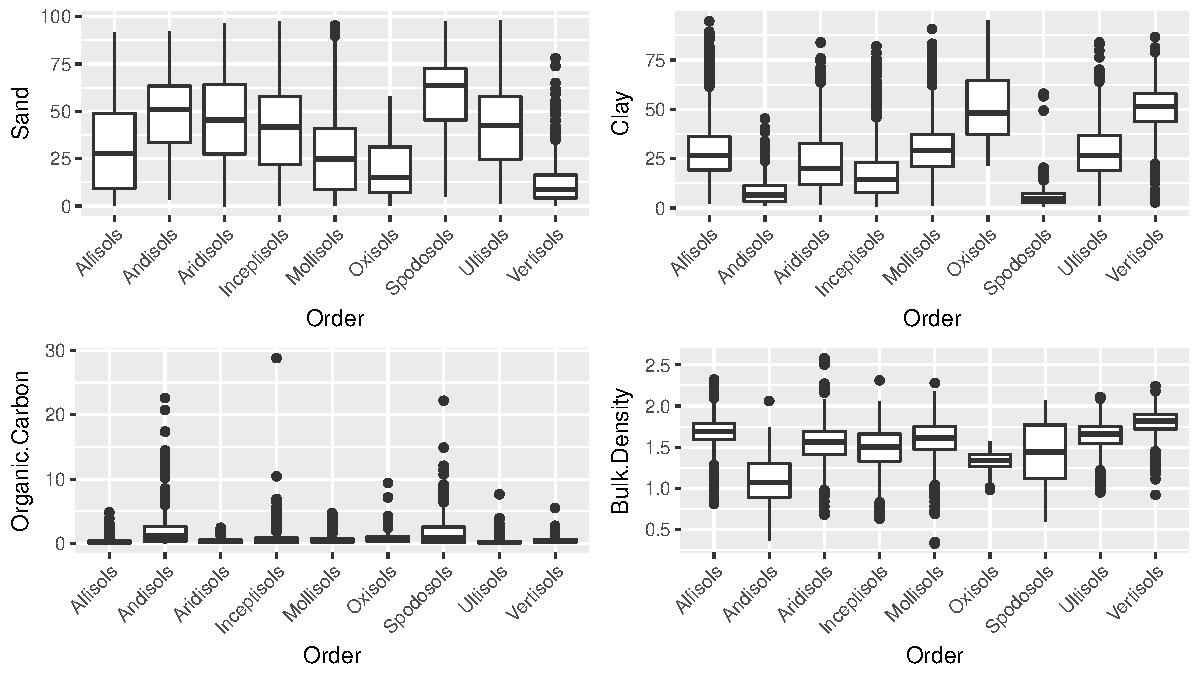
\includegraphics{Project4_files/figure-latex/EDA - Mer-1.pdf}
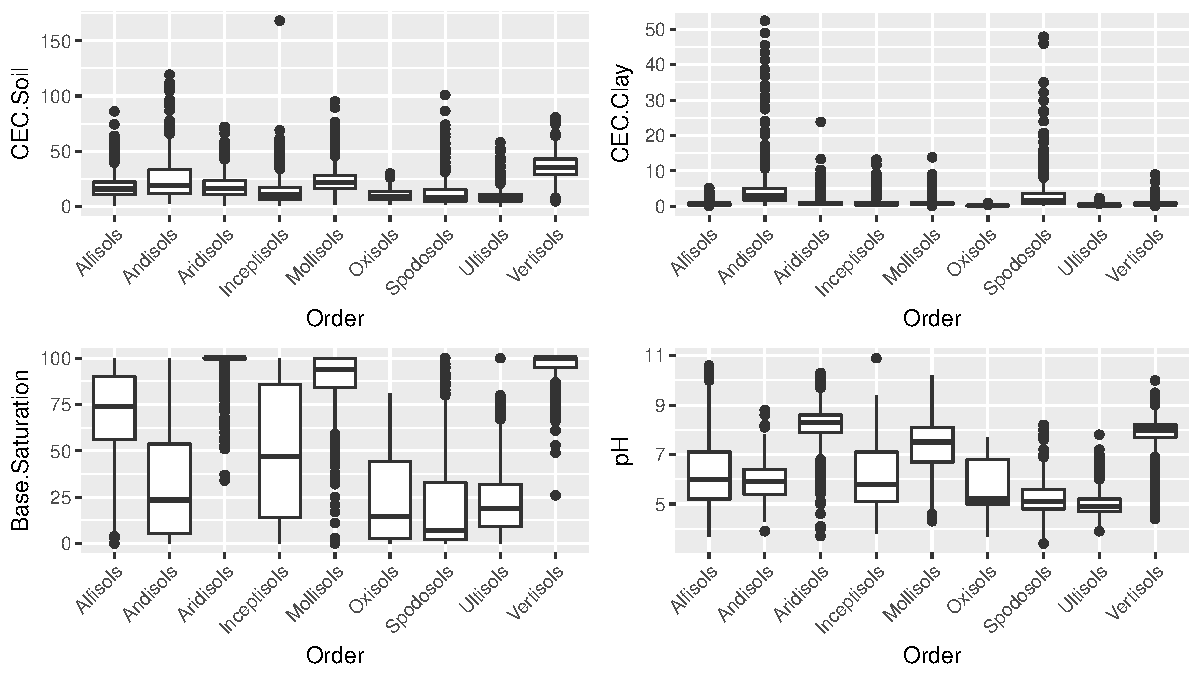
\includegraphics{Project4_files/figure-latex/EDA - Mer-2.pdf}

\section{Analysis}\label{analysis}

\section{EM Algorithm for Mixture of
Gaussians}\label{em-algorithm-for-mixture-of-gaussians}

In this application of an EM algorithm for a mixutre of Gaussians we
randomly divided our dataset to training data (70\%) and test data
(30\%). We applied the EM algorithm to training data to get the model
and then evaluated its accuracy in test data. Resulting plots and
precition confusion table are included below.

\begin{verbatim}
## Warning in plot.window(...): "alpha" is not a graphical parameter
\end{verbatim}

\begin{verbatim}
## Warning in plot.xy(xy, type, ...): "alpha" is not a graphical parameter
\end{verbatim}

\begin{verbatim}
## Warning in axis(side = side, at = at, labels = labels, ...): "alpha" is not
## a graphical parameter

## Warning in axis(side = side, at = at, labels = labels, ...): "alpha" is not
## a graphical parameter
\end{verbatim}

\begin{verbatim}
## Warning in box(...): "alpha" is not a graphical parameter
\end{verbatim}

\begin{verbatim}
## Warning in title(...): "alpha" is not a graphical parameter
\end{verbatim}

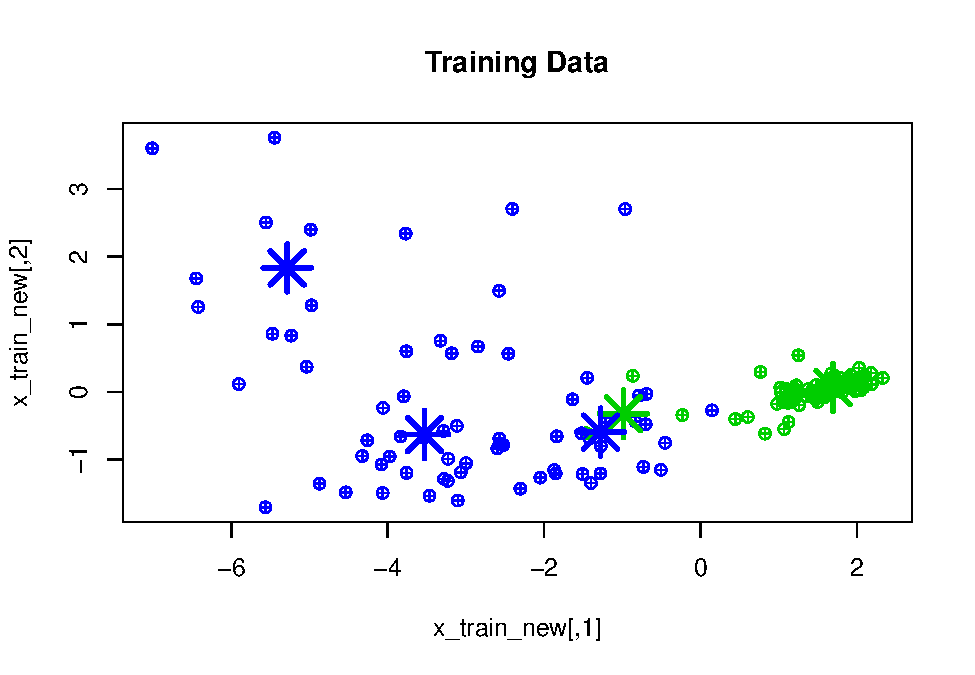
\includegraphics{Project4_files/figure-latex/EM applied to data-1.pdf}
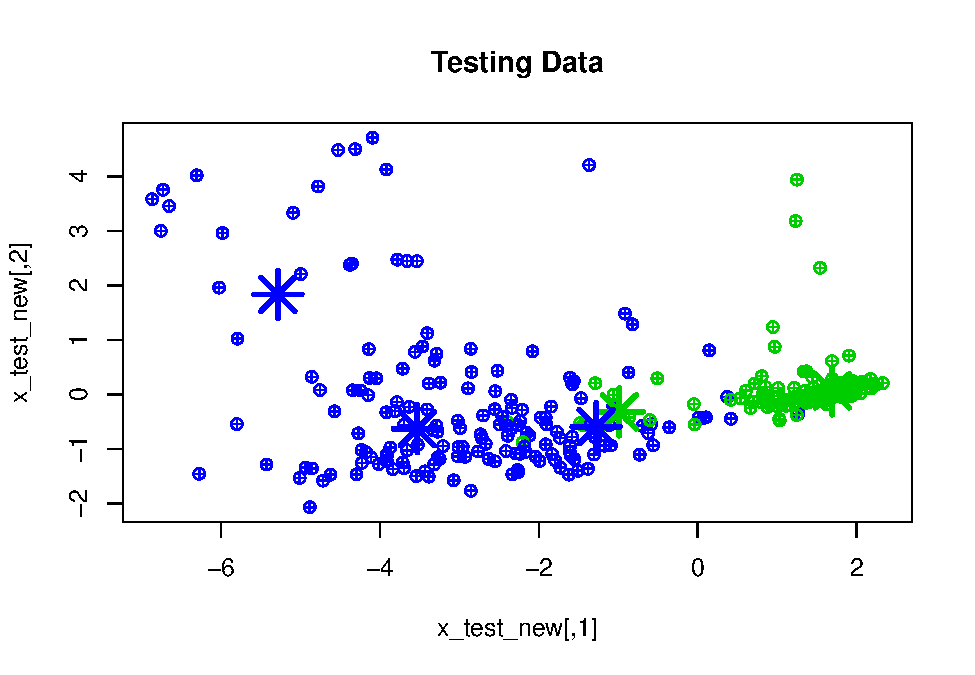
\includegraphics{Project4_files/figure-latex/EM applied to data-2.pdf}

\begin{longtable}[]{@{}lrr@{}}
\toprule
& benign & malignant\tabularnewline
\midrule
\endhead
benign & 298 & 6\tabularnewline
malignant & 11 & 164\tabularnewline
\#\# Comapriso & n between & MDA and Quadratic Discriminant Analysis
(QDA)\tabularnewline
\bottomrule
\end{longtable}

In this part of the analysis, we randomly divided our dataset to traning
data (80\%) and test data (20\%). We applied MDA in training data to get
the model and then evaluated its accuracy in test data. In order to test
the effects of the number of components in model performance and
elaborate the dilemma between model complexity and prediction accuracy,
we conducted MDA with the number of components included ranging from 2
to 8. The plot below shows the increasing prediction accuracy with the
increasing number of components included. Along with the number of
components increasing from 2 to 8, the predicting accuracy increased
from 50\% to 58\%. From a perspective of balancing model complexity and
prediction accuracy, we chose our final MDA model with four components
included and used that model to conduct following comparison with QDA
model.

In this analysis, we conducted MDA and QDA analysis based on the same
training and test dataset and the same first four components. The
prediction accuracy for each soil types and overall accuracy of these
two methods are shown in the table below. For the table we can see that
the overall accuracy of MDA and QDA are very similar (55\% for MDA and
54\% for QDA). However, their ability in correctly predicting individual
soil groups differed. For instance, MDA is better at Inceptisols and
Mollisols while QDA is better at Aridisols and Vertisols.

\begin{longtable}[]{@{}lrrrrrrrrrr@{}}
\toprule
& Alfisols & Andisols & Aridisols & Inceptisols & Mollisols & Oxisols &
Spodosols & Ultisols & Vertisols & Overall\tabularnewline
\midrule
\endhead
MDA & 0.53 & 0.34 & 0.42 & 0.24 & 0.72 & 0.47 & 0.41 & 0.69 & 0.55 &
0.55\tabularnewline
QDA & 0.51 & 0.31 & 0.65 & 0.05 & 0.58 & 0.35 & 0.56 & 0.76 & 0.68 &
0.54\tabularnewline
\bottomrule
\end{longtable}

\section{Conclusion}\label{conclusion}

In this project, we finished up two part.

In the first part, we coded a EM algorithm for mixed Gaussians and
applied it to a breast cancer dataset. Code for the EM functions are
included in the Appendix below.

In the second part, we conducted MDA on our dataset and explored the
increasing prediction accuracy with the increasing model complexity.
Through comparison with QDA on the same dataset using same predictors,
we found out the comparably acceptable performance of these two methods.

\section{Contributions}\label{contributions}

The different tasks required to complete this project were equally
divided between Meridith and Fei. Both members of this group contributed
to the presentation slides and this report.

\subsection{Appendix}\label{appendix}

\begin{Shaded}
\begin{Highlighting}[]
\KeywordTok{library}\NormalTok{(ggplot2)}
\KeywordTok{library}\NormalTok{(DAAG)}
\KeywordTok{library}\NormalTok{(dplyr)}
\KeywordTok{library}\NormalTok{(magrittr)}
\KeywordTok{library}\NormalTok{(MASS)}
\KeywordTok{library}\NormalTok{(caret)}
\KeywordTok{library}\NormalTok{(nnet) }
\KeywordTok{library}\NormalTok{(scales)}
\KeywordTok{library}\NormalTok{(klaR)}
\KeywordTok{library}\NormalTok{(stats)}
\KeywordTok{library}\NormalTok{(grid)}
\KeywordTok{library}\NormalTok{(gridExtra)}
\KeywordTok{library}\NormalTok{(mclust)}
\KeywordTok{library}\NormalTok{(mvtnorm)}
\KeywordTok{library}\NormalTok{(mda)}


\NormalTok{### split data into test and training sets}
\CommentTok{# df:         data set}
\CommentTok{# train_amt:  proportion of data to use for training}
\CommentTok{# resp_idx:   which column the class variable is (for breast cancer data this is 10)}
\NormalTok{split_data <-}\StringTok{ }\ControlFlowTok{function}\NormalTok{(df, train_amt, resp_idx) \{}
\NormalTok{  N <-}\StringTok{ }\KeywordTok{floor}\NormalTok{(}\KeywordTok{nrow}\NormalTok{(df) }\OperatorTok{*}\StringTok{ }\NormalTok{train_amt)}
\NormalTok{  ind <-}\StringTok{ }\KeywordTok{sample.int}\NormalTok{(}\KeywordTok{nrow}\NormalTok{(df), }\DataTypeTok{size =}\NormalTok{ N)}
\NormalTok{  x_train <-}\StringTok{ }\KeywordTok{as.matrix}\NormalTok{(df[ind,}\OperatorTok{-}\NormalTok{resp_idx])}
\NormalTok{  x_test <-}\StringTok{ }\KeywordTok{as.matrix}\NormalTok{(df[}\OperatorTok{-}\NormalTok{ind,}\OperatorTok{-}\NormalTok{resp_idx])}
\NormalTok{  class_train <-}\StringTok{ }\NormalTok{df[ind,resp_idx]}
\NormalTok{  class_test <-}\StringTok{ }\NormalTok{df[}\OperatorTok{-}\NormalTok{ind,resp_idx]}
  \KeywordTok{return}\NormalTok{(}\KeywordTok{list}\NormalTok{(}\DataTypeTok{x_train =}\NormalTok{ x_train,}
              \DataTypeTok{x_test =}\NormalTok{ x_test,}
              \DataTypeTok{class_train =}\NormalTok{ class_train,}
              \DataTypeTok{class_test =}\NormalTok{ class_test))}
\NormalTok{\}}

\NormalTok{### EM algorithm}
\CommentTok{# x:      covariates (as a matrix, one row = one observation)}
\CommentTok{# y:      response (as a factor)}
\CommentTok{# R:      number of subclasses for each class}
\CommentTok{# tol:    condition for convergence}
\CommentTok{# maxit:  maximum number of iterations for EM to run}
\NormalTok{EM <-}\StringTok{ }\ControlFlowTok{function}\NormalTok{(x, y, R, }\DataTypeTok{tol =} \FloatTok{1e-6}\NormalTok{, }\DataTypeTok{maxit =} \DecValTok{10}\NormalTok{) \{}
\NormalTok{  labs <-}\StringTok{ }\KeywordTok{levels}\NormalTok{(y)}
\NormalTok{  K <-}\StringTok{ }\KeywordTok{length}\NormalTok{(labs)}
\NormalTok{  M <-}\StringTok{ }\KeywordTok{ncol}\NormalTok{(x)}
\NormalTok{  N <-}\StringTok{ }\KeywordTok{nrow}\NormalTok{(x)}
\NormalTok{  pi <-}\StringTok{ }\KeywordTok{array}\NormalTok{(}\DecValTok{0}\NormalTok{, }\DataTypeTok{dim =} \KeywordTok{c}\NormalTok{(K, R))}
\NormalTok{  mu <-}\StringTok{ }\KeywordTok{array}\NormalTok{(}\DecValTok{0}\NormalTok{, }\DataTypeTok{dim =} \KeywordTok{c}\NormalTok{(K, M, R))}
\NormalTok{  sigma <-}\StringTok{ }\KeywordTok{diag}\NormalTok{(M)}
\NormalTok{  y <-}\StringTok{ }\KeywordTok{as.numeric}\NormalTok{(y)}
\NormalTok{  ### come up with starting points using kmeans}
  \ControlFlowTok{for}\NormalTok{(k }\ControlFlowTok{in} \DecValTok{1}\OperatorTok{:}\NormalTok{K) \{}
\NormalTok{    ind <-}\StringTok{ }\KeywordTok{which}\NormalTok{(y }\OperatorTok{==}\StringTok{ }\NormalTok{k)}
\NormalTok{    mu[k, , ] <-}\StringTok{ }\KeywordTok{t}\NormalTok{(}\KeywordTok{kmeans}\NormalTok{(x[ind, ], R)}\OperatorTok{$}\NormalTok{centers)}
\NormalTok{    pi[k, ] <-}\StringTok{ }\KeywordTok{rep}\NormalTok{(}\DecValTok{1}\OperatorTok{/}\NormalTok{R, }\DataTypeTok{length =}\NormalTok{ R)}
\NormalTok{  \}}
\NormalTok{  converged <-}\StringTok{ }\NormalTok{F}
\NormalTok{  ### main EM loop}
  \CommentTok{# while(!converged) \{}
  \ControlFlowTok{for}\NormalTok{(it }\ControlFlowTok{in} \DecValTok{1}\OperatorTok{:}\NormalTok{maxit) \{}
    \CommentTok{# E step}
\NormalTok{    p <-}\StringTok{ }\KeywordTok{array}\NormalTok{(}\DecValTok{0}\NormalTok{, }\DataTypeTok{dim =} \KeywordTok{c}\NormalTok{(N, R))}
    \ControlFlowTok{for}\NormalTok{(i }\ControlFlowTok{in} \DecValTok{1}\OperatorTok{:}\NormalTok{N) \{}
\NormalTok{      k <-}\StringTok{ }\NormalTok{y[i]}
      \ControlFlowTok{for}\NormalTok{(r }\ControlFlowTok{in} \DecValTok{1}\OperatorTok{:}\NormalTok{R) \{}
\NormalTok{        p[i,r] <-}\StringTok{ }\NormalTok{pi[k,r] }\OperatorTok{*}\StringTok{ }\KeywordTok{dmvnorm}\NormalTok{(x[i, ], mu[k, ,r], sigma)}
\NormalTok{      \}}
\NormalTok{      p[i, ] <-}\StringTok{ }\NormalTok{p[i, ]}\OperatorTok{/}\KeywordTok{sum}\NormalTok{(p[i, ])}
\NormalTok{    \}}
    \CommentTok{# M step}
    \ControlFlowTok{for}\NormalTok{(k }\ControlFlowTok{in} \DecValTok{1}\OperatorTok{:}\NormalTok{K) \{}
\NormalTok{      ind <-}\StringTok{ }\KeywordTok{which}\NormalTok{(y }\OperatorTok{==}\StringTok{ }\NormalTok{k)}
      \ControlFlowTok{for}\NormalTok{(r }\ControlFlowTok{in} \DecValTok{1}\OperatorTok{:}\NormalTok{R) \{}
\NormalTok{        pi[k,r] <-}\StringTok{ }\KeywordTok{sum}\NormalTok{(p[ind,r])}\OperatorTok{/}\KeywordTok{length}\NormalTok{(ind)}
\NormalTok{        mu[k, ,r] <-}\StringTok{ }\KeywordTok{colSums}\NormalTok{(x[ind, ]}\OperatorTok{*}\NormalTok{p[ind,r])}\OperatorTok{/}\KeywordTok{sum}\NormalTok{(p[ind,r])}
\NormalTok{      \}}
\NormalTok{    \}}
\NormalTok{    tally <-}\StringTok{ }\DecValTok{0}
    \ControlFlowTok{for}\NormalTok{(i }\ControlFlowTok{in} \DecValTok{1}\OperatorTok{:}\NormalTok{N) \{}
\NormalTok{      z <-}\StringTok{ }\NormalTok{y[i]}
      \ControlFlowTok{for}\NormalTok{(r }\ControlFlowTok{in} \DecValTok{1}\OperatorTok{:}\NormalTok{R) \{}
\NormalTok{        tmp <-}\StringTok{ }\NormalTok{x[i, ] }\OperatorTok{-}\StringTok{ }\NormalTok{mu[z, ,r]}
\NormalTok{        tally <-}\StringTok{ }\NormalTok{tally }\OperatorTok{+}\StringTok{ }\NormalTok{p[i,r] }\OperatorTok{*}\StringTok{ }\NormalTok{(tmp }\OperatorTok\StringTok{ }\NormalTok{tmp)}
\NormalTok{      \}}
\NormalTok{    \}}
\NormalTok{    sigma <-}\StringTok{ }\NormalTok{tally}\OperatorTok{/}\NormalTok{N}
    \CommentTok{# check convergence}

\NormalTok{  \}}
  \KeywordTok{return}\NormalTok{(}\KeywordTok{list}\NormalTok{(}\DataTypeTok{pi =}\NormalTok{ pi,}
              \DataTypeTok{mu =}\NormalTok{ mu,}
              \DataTypeTok{sigma =}\NormalTok{ sigma,}
              \DataTypeTok{class_labels =}\NormalTok{ labs))}
\NormalTok{\}}

\NormalTok{### predict classes}
\CommentTok{# em: object from the result of EM function above}
\CommentTok{# x: new data (as a matrix, one row = one observation)}
\NormalTok{em_predict <-}\StringTok{ }\ControlFlowTok{function}\NormalTok{(em, x) \{}
\NormalTok{  pi <-}\StringTok{ }\NormalTok{em}\OperatorTok{$}\NormalTok{pi}
\NormalTok{  mu <-}\StringTok{ }\NormalTok{em}\OperatorTok{$}\NormalTok{mu}
\NormalTok{  sigma <-}\StringTok{ }\NormalTok{em}\OperatorTok{$}\NormalTok{sigma}
\NormalTok{  labs <-}\StringTok{ }\NormalTok{em}\OperatorTok{$}\NormalTok{class_labels}
\NormalTok{  K <-}\StringTok{ }\KeywordTok{dim}\NormalTok{(mu)[}\DecValTok{1}\NormalTok{]}
\NormalTok{  R <-}\StringTok{ }\KeywordTok{dim}\NormalTok{(mu)[}\DecValTok{3}\NormalTok{]}
\NormalTok{  classes <-}\StringTok{ }\KeywordTok{rep}\NormalTok{(}\OtherTok{NA}\NormalTok{, }\KeywordTok{nrow}\NormalTok{(x))}

  \ControlFlowTok{for}\NormalTok{(i }\ControlFlowTok{in} \DecValTok{1}\OperatorTok{:}\KeywordTok{nrow}\NormalTok{(x)) \{}
\NormalTok{    probs <-}\StringTok{ }\KeywordTok{rep}\NormalTok{(}\DecValTok{0}\NormalTok{, K)}
    \ControlFlowTok{for}\NormalTok{(k }\ControlFlowTok{in} \DecValTok{1}\OperatorTok{:}\NormalTok{K) \{}
      \ControlFlowTok{for}\NormalTok{(r }\ControlFlowTok{in} \DecValTok{1}\OperatorTok{:}\NormalTok{R) \{}
\NormalTok{        probs[k] <-}\StringTok{ }\NormalTok{probs[k] }\OperatorTok{+}\StringTok{ }\NormalTok{pi[k,r] }\OperatorTok{*}\StringTok{ }\KeywordTok{dmvnorm}\NormalTok{(x[i, ], }\DataTypeTok{mean =}\NormalTok{ mu[k, ,r], }\DataTypeTok{sigma =}\NormalTok{ sigma)}
\NormalTok{      \}}
\NormalTok{    \}}
\NormalTok{    classes[i] <-}\StringTok{ }\KeywordTok{which.max}\NormalTok{(probs)}
\NormalTok{  \}}
  \KeywordTok{return}\NormalTok{(}\KeywordTok{factor}\NormalTok{(classes, }\DataTypeTok{labels =}\NormalTok{ labs))}
\NormalTok{\}}
\CommentTok{#EM data}
\CommentTok{# read data in and format it}
\NormalTok{data <-}\StringTok{ }\KeywordTok{read.csv}\NormalTok{(}\StringTok{'http://archive.ics.uci.edu/ml/machine-learning-databases/breast-cancer-wisconsin/breast-cancer-wisconsin.data'}\NormalTok{, }\DataTypeTok{header =}\NormalTok{ F, }\DataTypeTok{na.strings =} \StringTok{'?'}\NormalTok{)}
\KeywordTok{names}\NormalTok{(data) <-}\StringTok{ }\KeywordTok{c}\NormalTok{(}\StringTok{'id'}\NormalTok{,}\StringTok{'thickness'}\NormalTok{,}\StringTok{'size.unif'}\NormalTok{,}\StringTok{'shape.unif'}\NormalTok{,}\StringTok{'adhesion'}\NormalTok{,}\StringTok{'size.cell'}\NormalTok{,}\StringTok{'nuclei'}\NormalTok{,}\StringTok{'chromatin'}\NormalTok{,}\StringTok{'nucleoli'}\NormalTok{,}\StringTok{'mitoses'}\NormalTok{,}\StringTok{'class'}\NormalTok{)}
\NormalTok{data}\OperatorTok{$}\NormalTok{class <-}\StringTok{ }\KeywordTok{as.factor}\NormalTok{(data}\OperatorTok{$}\NormalTok{class)}
\KeywordTok{levels}\NormalTok{(data}\OperatorTok{$}\NormalTok{class) <-}\StringTok{ }\KeywordTok{c}\NormalTok{(}\StringTok{'benign'}\NormalTok{,}\StringTok{'malignant'}\NormalTok{)}
\NormalTok{data <-}\StringTok{ }\NormalTok{data[}\OperatorTok{-}\KeywordTok{which}\NormalTok{(}\KeywordTok{is.na}\NormalTok{(data}\OperatorTok{$}\NormalTok{nuclei)),}\OperatorTok{-}\DecValTok{1}\NormalTok{] }\CommentTok{# leave ID column out and remove NAs}


\CommentTok{# Basic clearning of our dataset }
\NormalTok{project1data <-}\StringTok{ }\KeywordTok{read.csv}\NormalTok{(}\DataTypeTok{file =} \StringTok{"project1data.csv"}\NormalTok{)}
\NormalTok{project1data <-}\StringTok{ }\NormalTok{project1data[,}\OperatorTok{-}\KeywordTok{c}\NormalTok{(}\DecValTok{1}\NormalTok{,}\DecValTok{2}\NormalTok{,}\DecValTok{4}\NormalTok{)] }\CommentTok{#remove the ID and Horizon columns which are useless,Silt is redundant information since it could be calculated from Sand and Clay. }
\NormalTok{project1data <-}\StringTok{ }\NormalTok{project1data[}\KeywordTok{sample}\NormalTok{(}\KeywordTok{nrow}\NormalTok{(project1data),}\KeywordTok{nrow}\NormalTok{(project1data)),] ###shuffle rows}



\NormalTok{varlist <-}\StringTok{ }\KeywordTok{names}\NormalTok{(project1data)[}\OperatorTok{-}\DecValTok{9}\NormalTok{]}

\NormalTok{customPlot <-}\StringTok{ }\ControlFlowTok{function}\NormalTok{(varName) \{}

\NormalTok{project1data }\OperatorTok\StringTok{ }
\KeywordTok{group_by_}\NormalTok{(}\StringTok{"Order"}\NormalTok{) }\OperatorTok\StringTok{ }
\KeywordTok{select_}\NormalTok{(}\StringTok{"Order"}\NormalTok{,varName) }\OperatorTok\StringTok{ }
\KeywordTok{ggplot}\NormalTok{(}\KeywordTok{aes_string}\NormalTok{(}\StringTok{"Order"}\NormalTok{,varName)) }\OperatorTok{+}\StringTok{ }\KeywordTok{geom_boxplot}\NormalTok{() }\OperatorTok{+}\StringTok{ }
\StringTok{   }\KeywordTok{theme}\NormalTok{(}\DataTypeTok{axis.text.x =} \KeywordTok{element_text}\NormalTok{(}\DataTypeTok{angle =} \DecValTok{45}\NormalTok{, }\DataTypeTok{hjust =} \DecValTok{1}\NormalTok{))}

\NormalTok{\}}

\KeywordTok{grid.arrange}\NormalTok{(}\DataTypeTok{grobs =} \KeywordTok{lapply}\NormalTok{(varlist[}\DecValTok{1}\OperatorTok{:}\DecValTok{4}\NormalTok{],customPlot))}
\KeywordTok{grid.arrange}\NormalTok{(}\DataTypeTok{grobs =} \KeywordTok{lapply}\NormalTok{(varlist[}\DecValTok{5}\OperatorTok{:}\DecValTok{8}\NormalTok{],customPlot))}


\CommentTok{# pairs(project1data)}
\CommentTok{# cor(project1data[, -9])}



\CommentTok{# Create new dataset with PCA }
\NormalTok{pca =}\StringTok{ }\KeywordTok{prcomp}\NormalTok{(project1data[,}\OperatorTok{-}\DecValTok{9}\NormalTok{])}
\CommentTok{# print(pca$rotation)}
\NormalTok{summary.pca =}\StringTok{ }\KeywordTok{summary}\NormalTok{(pca)}
\CommentTok{# print(summary.pca)}
\NormalTok{project1data.new =}\StringTok{ }\KeywordTok{data.frame}\NormalTok{(}\DataTypeTok{pca=}\NormalTok{pca}\OperatorTok{$}\NormalTok{x[,}\DecValTok{1}\OperatorTok{:}\DecValTok{8}\NormalTok{],}\DataTypeTok{Order=}\NormalTok{project1data}\OperatorTok{$}\NormalTok{Order) }

\CommentTok{#table of the variance and coefficients}
\CommentTok{#knitr::kable(summary.pca$importance)}
\CommentTok{#knitr::kable(pca$rotation[, 1:4])}


\CommentTok{#data partition}
\NormalTok{train_id <-}\StringTok{ }\NormalTok{caret}\OperatorTok{::}\KeywordTok{createDataPartition}\NormalTok{(}\DataTypeTok{y=}\NormalTok{project1data.new}\OperatorTok{$}\NormalTok{Order, }\DataTypeTok{p=}\FloatTok{0.8}\NormalTok{,}\DataTypeTok{list =} \OtherTok{FALSE}\NormalTok{)}
\NormalTok{train <-}\StringTok{ }\NormalTok{project1data.new[train_id,]}
\NormalTok{test <-}\StringTok{ }\NormalTok{project1data.new[}\OperatorTok{-}\NormalTok{train_id,]}
\CommentTok{# Mixture Discriminant Analysis (MDA)}






\NormalTok{R <-}\StringTok{ }\DecValTok{3} \CommentTok{# number of subclasses}
\NormalTok{training_amount <-}\StringTok{ }\FloatTok{0.3}

\NormalTok{X <-}\StringTok{ }\KeywordTok{split_data}\NormalTok{(data, training_amount, }\DecValTok{10}\NormalTok{)}
\NormalTok{x_train <-}\StringTok{ }\NormalTok{X}\OperatorTok{$}\NormalTok{x_train}
\NormalTok{x_test <-}\StringTok{ }\NormalTok{X}\OperatorTok{$}\NormalTok{x_test}
\NormalTok{class_train <-}\StringTok{ }\NormalTok{X}\OperatorTok{$}\NormalTok{class_train}
\NormalTok{class_test <-}\StringTok{ }\NormalTok{X}\OperatorTok{$}\NormalTok{class_test}

\CommentTok{# run MDA}
\NormalTok{fit <-}\StringTok{ }\KeywordTok{EM}\NormalTok{(x_train, class_train, R)}
\CommentTok{# classify test data}
\NormalTok{fit_pred <-}\StringTok{ }\KeywordTok{em_predict}\NormalTok{(fit, x_test)}
\CommentTok{# resulting confusion matrix and error rate}
\CommentTok{# confusion(fit_pred, class_test)}

\CommentTok{# try PCA}
\NormalTok{x <-}\StringTok{ }\KeywordTok{rbind}\NormalTok{(x_train, x_test)}
\NormalTok{x_scaled <-}\StringTok{ }\KeywordTok{apply}\NormalTok{(x, }\DecValTok{2}\NormalTok{, }\ControlFlowTok{function}\NormalTok{(x) (x }\OperatorTok{-}\StringTok{ }\KeywordTok{mean}\NormalTok{(x))}\OperatorTok{/}\KeywordTok{sd}\NormalTok{(x))}
\NormalTok{eig <-}\StringTok{ }\KeywordTok{eigen}\NormalTok{(}\KeywordTok{cov}\NormalTok{(x_scaled))}
\CommentTok{# eig$values/sum(eig$values)}
\NormalTok{V <-}\StringTok{ }\NormalTok{eig}\OperatorTok{$}\NormalTok{vectors[ ,}\DecValTok{1}\OperatorTok{:}\DecValTok{2}\NormalTok{]}
\NormalTok{x_new <-}\StringTok{ }\KeywordTok{as.matrix}\NormalTok{(x_scaled }\OperatorTok\StringTok{ }\NormalTok{V)}
\NormalTok{x_train_new <-}\StringTok{ }\NormalTok{x_new[}\DecValTok{1}\OperatorTok{:}\KeywordTok{nrow}\NormalTok{(x_train), ]}
\NormalTok{x_test_new <-}\StringTok{ }\NormalTok{x_new[}\OperatorTok{-}\NormalTok{(}\DecValTok{1}\OperatorTok{:}\KeywordTok{nrow}\NormalTok{(x_train)), ]}

\NormalTok{fit2 <-}\StringTok{ }\KeywordTok{EM}\NormalTok{(x_train_new, class_train, R)}
\NormalTok{fit_pred2 <-}\StringTok{ }\KeywordTok{em_predict}\NormalTok{(fit2, x_test_new)}
\CommentTok{# confusion(fit_pred2, class_test)}

\CommentTok{#training plot}
\KeywordTok{plot}\NormalTok{(x_train_new, }\DataTypeTok{pch =} \DecValTok{10}\NormalTok{, }\DataTypeTok{alpha =} \FloatTok{0.5}\NormalTok{, }\DataTypeTok{col =} \KeywordTok{as.numeric}\NormalTok{(class_train)}\OperatorTok{+}\DecValTok{2}\NormalTok{, }
      \DataTypeTok{main =} \StringTok{"Training Data"}\NormalTok{)}
\KeywordTok{points}\NormalTok{(}\KeywordTok{t}\NormalTok{(fit2}\OperatorTok{$}\NormalTok{mu[}\DecValTok{1}\NormalTok{, , ]), }\DataTypeTok{pch =} \DecValTok{8}\NormalTok{, }\DataTypeTok{cex =} \DecValTok{3}\NormalTok{, }\DataTypeTok{lwd =} \DecValTok{3}\NormalTok{, }\DataTypeTok{col =} \DecValTok{3}\NormalTok{)}
\KeywordTok{points}\NormalTok{(}\KeywordTok{t}\NormalTok{(fit2}\OperatorTok{$}\NormalTok{mu[}\DecValTok{2}\NormalTok{, , ]), }\DataTypeTok{pch =} \DecValTok{8}\NormalTok{, }\DataTypeTok{cex =} \DecValTok{3}\NormalTok{, }\DataTypeTok{lwd =} \DecValTok{3}\NormalTok{, }\DataTypeTok{col =} \DecValTok{4}\NormalTok{)}
\CommentTok{#testing plot}
\KeywordTok{plot}\NormalTok{(x_test_new, }\DataTypeTok{pch =} \DecValTok{10}\NormalTok{, }\DataTypeTok{col =} \KeywordTok{as.numeric}\NormalTok{(class_test)}\OperatorTok{+}\DecValTok{2}\NormalTok{,}
     \DataTypeTok{main =} \StringTok{"Testing Data"}\NormalTok{)}
\KeywordTok{points}\NormalTok{(}\KeywordTok{t}\NormalTok{(fit2}\OperatorTok{$}\NormalTok{mu[}\DecValTok{1}\NormalTok{, , ]), }\DataTypeTok{pch =} \DecValTok{8}\NormalTok{, }\DataTypeTok{cex =} \DecValTok{3}\NormalTok{, }\DataTypeTok{lwd =} \DecValTok{3}\NormalTok{, }\DataTypeTok{col =} \DecValTok{3}\NormalTok{)}
\KeywordTok{points}\NormalTok{(}\KeywordTok{t}\NormalTok{(fit2}\OperatorTok{$}\NormalTok{mu[}\DecValTok{2}\NormalTok{, , ]), }\DataTypeTok{pch =} \DecValTok{8}\NormalTok{, }\DataTypeTok{cex =} \DecValTok{3}\NormalTok{, }\DataTypeTok{lwd =} \DecValTok{3}\NormalTok{, }\DataTypeTok{col =} \DecValTok{4}\NormalTok{)}



\NormalTok{knitr}\OperatorTok{::}\KeywordTok{kable}\NormalTok{(}\KeywordTok{table}\NormalTok{(fit_pred2, class_test))}


\CommentTok{#mda - 2 component }
\NormalTok{mda.}\DecValTok{2}\NormalTok{ <-}\StringTok{ }\KeywordTok{mda}\NormalTok{(Order }\OperatorTok{~}\StringTok{ }\NormalTok{pca.PC1 }\OperatorTok{+}\StringTok{ }\NormalTok{pca.PC2 , }\DataTypeTok{data =}\NormalTok{ train)}
\CommentTok{#predict test data}
\NormalTok{mda2.predict =}\StringTok{ }\KeywordTok{predict}\NormalTok{(mda.}\DecValTok{2}\NormalTok{, }\DataTypeTok{newdata=}\NormalTok{test)}
\CommentTok{# Assess the total accuracy of test data}
\NormalTok{ct2.mda <-}\StringTok{ }\KeywordTok{table}\NormalTok{(test}\OperatorTok{$}\NormalTok{Order, mda2.predict)}
\NormalTok{totcorrect2.mda <-}\StringTok{ }\KeywordTok{sum}\NormalTok{(}\KeywordTok{diag}\NormalTok{(}\KeywordTok{prop.table}\NormalTok{(ct2.mda)))}
\CommentTok{# Assess the accuracy of the prediction for each soil class (Order) in test data}
\CommentTok{#cc2.mda <- diag(prop.table(ct2.mda, 1))}

\CommentTok{#mda - 3 component }
\NormalTok{mda.}\DecValTok{3}\NormalTok{ <-}\StringTok{ }\KeywordTok{mda}\NormalTok{(Order }\OperatorTok{~}\StringTok{ }\NormalTok{pca.PC1 }\OperatorTok{+}\StringTok{ }\NormalTok{pca.PC2}\OperatorTok{+}\StringTok{ }\NormalTok{pca.PC3 , }\DataTypeTok{data =}\NormalTok{ train)}
\CommentTok{#predict test data}
\NormalTok{mda3.predict =}\StringTok{ }\KeywordTok{predict}\NormalTok{(mda.}\DecValTok{3}\NormalTok{, }\DataTypeTok{newdata=}\NormalTok{test)}
\CommentTok{# Assess the total accuracy of test data}
\NormalTok{ct3.mda <-}\StringTok{ }\KeywordTok{table}\NormalTok{(test}\OperatorTok{$}\NormalTok{Order, mda3.predict)}
\NormalTok{totcorrect3.mda <-}\StringTok{ }\KeywordTok{sum}\NormalTok{(}\KeywordTok{diag}\NormalTok{(}\KeywordTok{prop.table}\NormalTok{(ct3.mda)))}

\CommentTok{#mda - 4 component }
\NormalTok{mda.}\DecValTok{4}\NormalTok{ <-}\StringTok{ }\KeywordTok{mda}\NormalTok{(Order }\OperatorTok{~}\StringTok{ }\NormalTok{pca.PC1 }\OperatorTok{+}\StringTok{ }\NormalTok{pca.PC2}\OperatorTok{+}\StringTok{ }\NormalTok{pca.PC3}\OperatorTok{+}\StringTok{ }\NormalTok{pca.PC4 , }\DataTypeTok{data =}\NormalTok{ train)}
\CommentTok{#predict test data}
\NormalTok{mda4.predict =}\StringTok{ }\KeywordTok{predict}\NormalTok{(mda.}\DecValTok{4}\NormalTok{, }\DataTypeTok{newdata=}\NormalTok{test)}
\CommentTok{# Assess the total accuracy of test data}
\NormalTok{ct4.mda <-}\StringTok{ }\KeywordTok{table}\NormalTok{(test}\OperatorTok{$}\NormalTok{Order, mda4.predict)}
\NormalTok{totcorrect4.mda <-}\StringTok{ }\KeywordTok{sum}\NormalTok{(}\KeywordTok{diag}\NormalTok{(}\KeywordTok{prop.table}\NormalTok{(ct4.mda)))}

\CommentTok{#mda - 5 component }
\NormalTok{mda.}\DecValTok{5}\NormalTok{ <-}\StringTok{ }\KeywordTok{mda}\NormalTok{(Order }\OperatorTok{~}\StringTok{ }\NormalTok{pca.PC1 }\OperatorTok{+}\StringTok{ }\NormalTok{pca.PC2}\OperatorTok{+}\StringTok{ }\NormalTok{pca.PC3}\OperatorTok{+}\StringTok{ }\NormalTok{pca.PC4 }\OperatorTok{+}\StringTok{ }\NormalTok{pca.PC5, }\DataTypeTok{data =}\NormalTok{ train)}
\CommentTok{#predict test data}
\NormalTok{mda5.predict =}\StringTok{ }\KeywordTok{predict}\NormalTok{(mda.}\DecValTok{5}\NormalTok{, }\DataTypeTok{newdata=}\NormalTok{test)}
\CommentTok{# Assess the total accuracy of test data}
\NormalTok{ct5.mda <-}\StringTok{ }\KeywordTok{table}\NormalTok{(test}\OperatorTok{$}\NormalTok{Order, mda5.predict)}
\NormalTok{totcorrect5.mda <-}\StringTok{ }\KeywordTok{sum}\NormalTok{(}\KeywordTok{diag}\NormalTok{(}\KeywordTok{prop.table}\NormalTok{(ct5.mda)))}

\CommentTok{#mda - 6 component }
\NormalTok{mda.}\DecValTok{6}\NormalTok{ <-}\StringTok{ }\KeywordTok{mda}\NormalTok{(Order }\OperatorTok{~}\StringTok{ }\NormalTok{pca.PC1 }\OperatorTok{+}\StringTok{ }\NormalTok{pca.PC2}\OperatorTok{+}\StringTok{ }\NormalTok{pca.PC3}\OperatorTok{+}\StringTok{ }\NormalTok{pca.PC4 }\OperatorTok{+}\StringTok{ }\NormalTok{pca.PC5}\OperatorTok{+}\StringTok{ }\NormalTok{pca.PC6, }\DataTypeTok{data =}\NormalTok{ train)}
\CommentTok{#predict test data}
\NormalTok{mda6.predict =}\StringTok{ }\KeywordTok{predict}\NormalTok{(mda.}\DecValTok{6}\NormalTok{, }\DataTypeTok{newdata=}\NormalTok{test)}
\CommentTok{# Assess the total accuracy of test data}
\NormalTok{ct6.mda <-}\StringTok{ }\KeywordTok{table}\NormalTok{(test}\OperatorTok{$}\NormalTok{Order, mda6.predict)}
\NormalTok{totcorrect6.mda <-}\StringTok{ }\KeywordTok{sum}\NormalTok{(}\KeywordTok{diag}\NormalTok{(}\KeywordTok{prop.table}\NormalTok{(ct6.mda)))}

\CommentTok{#mda - 7 component }
\NormalTok{mda.}\DecValTok{7}\NormalTok{ <-}\StringTok{ }\KeywordTok{mda}\NormalTok{(Order }\OperatorTok{~}\StringTok{ }\NormalTok{pca.PC1 }\OperatorTok{+}\StringTok{ }\NormalTok{pca.PC2}\OperatorTok{+}\StringTok{ }\NormalTok{pca.PC3}\OperatorTok{+}\StringTok{ }\NormalTok{pca.PC4 }\OperatorTok{+}\StringTok{ }\NormalTok{pca.PC5}\OperatorTok{+}\StringTok{ }\NormalTok{pca.PC6}\OperatorTok{+}\StringTok{ }\NormalTok{pca.PC7, }\DataTypeTok{data =}\NormalTok{ train)}
\CommentTok{#predict test data}
\NormalTok{mda7.predict =}\StringTok{ }\KeywordTok{predict}\NormalTok{(mda.}\DecValTok{7}\NormalTok{, }\DataTypeTok{newdata=}\NormalTok{test)}
\CommentTok{# Assess the total accuracy of test data}
\NormalTok{ct7.mda <-}\StringTok{ }\KeywordTok{table}\NormalTok{(test}\OperatorTok{$}\NormalTok{Order, mda7.predict)}
\NormalTok{totcorrect7.mda <-}\StringTok{ }\KeywordTok{sum}\NormalTok{(}\KeywordTok{diag}\NormalTok{(}\KeywordTok{prop.table}\NormalTok{(ct7.mda)))}

\CommentTok{#mda - 8 component }
\NormalTok{mda.}\DecValTok{8}\NormalTok{ <-}\StringTok{ }\KeywordTok{mda}\NormalTok{(Order }\OperatorTok{~}\StringTok{ }\NormalTok{pca.PC1 }\OperatorTok{+}\StringTok{ }\NormalTok{pca.PC2}\OperatorTok{+}\StringTok{ }\NormalTok{pca.PC3}\OperatorTok{+}\StringTok{ }\NormalTok{pca.PC4 }\OperatorTok{+}\StringTok{ }\NormalTok{pca.PC5}\OperatorTok{+}\StringTok{ }\NormalTok{pca.PC6}\OperatorTok{+}\StringTok{ }\NormalTok{pca.PC7}\OperatorTok{+}\StringTok{ }\NormalTok{pca.PC8, }\DataTypeTok{data =}\NormalTok{ train)}
\CommentTok{#predict test data}
\NormalTok{mda8.predict =}\StringTok{ }\KeywordTok{predict}\NormalTok{(mda.}\DecValTok{8}\NormalTok{, }\DataTypeTok{newdata=}\NormalTok{test)}
\CommentTok{# Assess the total accuracy of test data}
\NormalTok{ct8.mda <-}\StringTok{ }\KeywordTok{table}\NormalTok{(test}\OperatorTok{$}\NormalTok{Order, mda8.predict)}
\NormalTok{totcorrect8.mda <-}\StringTok{ }\KeywordTok{sum}\NormalTok{(}\KeywordTok{diag}\NormalTok{(}\KeywordTok{prop.table}\NormalTok{(ct8.mda)))}


\CommentTok{#mda - 4 component }
\NormalTok{mda <-}\StringTok{ }\KeywordTok{mda}\NormalTok{(Order }\OperatorTok{~}\StringTok{ }\NormalTok{pca.PC1 }\OperatorTok{+}\StringTok{ }\NormalTok{pca.PC2}\OperatorTok{+}\StringTok{ }\NormalTok{pca.PC3}\OperatorTok{+}\StringTok{ }\NormalTok{pca.PC4 , }\DataTypeTok{data =}\NormalTok{ train)}
\CommentTok{#predict test data}
\NormalTok{mda.predict =}\StringTok{ }\KeywordTok{predict}\NormalTok{(mda, }\DataTypeTok{newdata=}\NormalTok{test)}
\CommentTok{# Assess the accuracy of the prediction for each soil class (Order) in test data}
\NormalTok{ct.mda <-}\StringTok{ }\KeywordTok{table}\NormalTok{(test}\OperatorTok{$}\NormalTok{Order, mda.predict)}
\NormalTok{cc.mda <-}\StringTok{ }\KeywordTok{diag}\NormalTok{(}\KeywordTok{prop.table}\NormalTok{(ct.mda, }\DecValTok{1}\NormalTok{))}
\CommentTok{# Assess the total accuracy of test data}
\NormalTok{totcorrect.mda <-}\StringTok{ }\KeywordTok{sum}\NormalTok{(}\KeywordTok{diag}\NormalTok{(}\KeywordTok{prop.table}\NormalTok{(ct4.mda)))}


\CommentTok{#qda}
\NormalTok{qda.fei <-}\StringTok{ }\NormalTok{MASS}\OperatorTok{::}\KeywordTok{qda}\NormalTok{(Order }\OperatorTok{~}\NormalTok{pca.PC1 }\OperatorTok{+}\StringTok{ }\NormalTok{pca.PC2}\OperatorTok{+}\StringTok{ }\NormalTok{pca.PC3}\OperatorTok{+}\StringTok{ }\NormalTok{pca.PC4, }\DataTypeTok{data =}\NormalTok{ train)}

\CommentTok{#predict test data}
\NormalTok{qda.predict =}\StringTok{ }\KeywordTok{predict}\NormalTok{(qda.fei, }\DataTypeTok{newdata=}\NormalTok{test)}

\CommentTok{# Assess the accuracy of the prediction for each soil class (Order) in test data}
\NormalTok{ct.qda <-}\StringTok{ }\KeywordTok{table}\NormalTok{(test}\OperatorTok{$}\NormalTok{Order, qda.predict}\OperatorTok{$}\NormalTok{class)}
\NormalTok{cc.qda <-}\StringTok{ }\KeywordTok{diag}\NormalTok{(}\KeywordTok{prop.table}\NormalTok{(ct.qda, }\DecValTok{1}\NormalTok{))}


\NormalTok{### comparison }
\CommentTok{#mda}
\NormalTok{correct.mda <-}\StringTok{ }\KeywordTok{diag}\NormalTok{(}\KeywordTok{prop.table}\NormalTok{(ct.mda, }\DecValTok{1}\NormalTok{))}
\CommentTok{# total percent correct}
\NormalTok{totcorrect.mda <-}\StringTok{ }\KeywordTok{sum}\NormalTok{(}\KeywordTok{diag}\NormalTok{(}\KeywordTok{prop.table}\NormalTok{(ct.mda)))}

\CommentTok{#qda}
\NormalTok{correct.qda <-}\StringTok{ }\KeywordTok{diag}\NormalTok{(}\KeywordTok{prop.table}\NormalTok{(ct.qda, }\DecValTok{1}\NormalTok{))}
\CommentTok{# total percent correct}
\NormalTok{totcorrect.qda <-}\StringTok{ }\KeywordTok{sum}\NormalTok{(}\KeywordTok{diag}\NormalTok{(}\KeywordTok{prop.table}\NormalTok{(ct.qda)))}


\NormalTok{##table }

\NormalTok{model_comparison <-}\StringTok{ }\KeywordTok{data.frame}\NormalTok{(}\KeywordTok{rbind}\NormalTok{(correct.mda, correct.qda))}
\NormalTok{model_comparison}\OperatorTok{$}\NormalTok{Overall=}\KeywordTok{c}\NormalTok{(totcorrect.mda,totcorrect.qda)}

\NormalTok{model_comparison <-model_comparison }\OperatorTok\KeywordTok{set_rownames}\NormalTok{(}\KeywordTok{c}\NormalTok{(}\StringTok{"MDA"}\NormalTok{, }\StringTok{"QDA"}\NormalTok{))}
\NormalTok{knitr}\OperatorTok{::}\KeywordTok{kable}\NormalTok{(}\KeywordTok{round}\NormalTok{(model_comparison, }\DataTypeTok{digits =} \DecValTok{2}\NormalTok{))}

\CommentTok{#p <- ggplot(test, aes(x = Sand, y = Clay, color = mda.predict)) + geom_point() + stat_contour(aes(x = Sand, y = Clay, z = mda.predict), data = test) + labs(title="MDA Decision Boundaries")}
\CommentTok{#p}
\end{Highlighting}
\end{Shaded}


\end{document}
